\documentclass[a4paper,11pt]{article}

% --- PAQUETES BÁSICOS ---
\usepackage[utf8]{inputenc}
\usepackage[spanish,es-tabla]{babel}
\usepackage[margin=17mm]{geometry}
\usepackage{amsmath}
\usepackage{amssymb}
\usepackage{graphicx}
\graphicspath{ {../examples/images/} }
\usepackage{booktabs}
\usepackage{cite}
\usepackage{microtype}
\usepackage{listings}
\usepackage{color}
%\usepackage{hyperref}
\usepackage[
    colorlinks=false,           % No colorear el texto, solo subrayar
    linkbordercolor={1 0 0},    % Color del subrayado (RGB: rojo)
    pdfborderstyle={/S/U/W 0.5}   % /S/U = underline, W = grosor (1pt)
]{hyperref}
\renewcommand{\lstlistingname}{Listado de código}


% --- CONFIGURACIÓN DE LISTINGS PARA PSEUDOCÓDIGO ---
\definecolor{codegray}{rgb}{0.5,0.5,0.5}
\definecolor{codeblue}{rgb}{0.13,0.13,1.0}
\lstset{
    backgroundcolor=\color{white},
    basicstyle=\ttfamily\small,
    breakatwhitespace=false,
    breaklines=true,
    captionpos=b,
    commentstyle=\color{codegray}\itshape,
    keepspaces=true,
    numbers=left,
    numbernumber=1,
    numbersep=8pt,
    numberstyle=\tiny\color{codegray},
    showspaces=false,
    showstringspaces=false,
    showtabs=false,
    tabsize=4,
    frame=single,
    rulecolor=\color{black},
    keywordstyle=\color{codeblue}\bfseries,
    morekeywords={Algoritmo,Entrada,Salida,Para,desde,hasta,hacer,Fin,Si,entonces,Sino,Mientras,Retornar,Copiar,promedio,desv_estandar,evaluar,ajustar,maximo,limitar_entre_valores,construir_matriz_diagonal,resolver_sistema_lineal}
}

% --- METADATOS ---
\title{\textbf{Informe de Desarrollo: \\Preprocesamiento de Espectros FTIR en Espacio de Absorbancia e Identificación Automática de Grupos Funcionales en GO y rGO}}
\author{\textbf{Matías Roberto Alemán}}
\date{8 de junio de 2026}

\begin{document}

\maketitle

\begin{abstract}
Este informe presenta el diseño matemático, algorítmico e ingenieril de un sistema automático de procesamiento y asignación de espectros de espectroscopía de infrarrojo por transformada de Fourier (FTIR) aplicado al Óxido de Grafeno (GO) y Óxido de Grafeno Reducido (rGO). Se describe la transición física del espacio de Transmitancia ($\%T$) al de Absorbancia ($A$), un espacio linealmente aditivo según la ley de Beer-Lambert que mejora sustancialmente la robustez del filtrado. Mediante un barrido paramétrico exhaustivo de 180 configuraciones de preprocesamiento, se analizan los efectos del suavizado y la remoción de línea base, logrando la detección de la totalidad de las bandas analíticas clave. Finalmente, se presentan informes cuantitativos y una discusión fisicoquímica del proceso de reducción de los grupos oxigenados en la nanoestructura grafénica.
\end{abstract}

\tableofcontents

\newpage

% ==========================================
\section{Introducción y Fundamentos Físicos}
% ==========================================
El Óxido de Grafeno (GO) es un nanomaterial de carbono bidimensional caracterizado por una alta densidad de grupos funcionales que contienen oxígeno, tales como hidroxilos, epoxilos, carbonilos y carboxilos, los cuales decoran su plano basal y bordes. El proceso de reducción química o térmica del GO para producir Óxido de Grafeno Reducido (rGO) remueve la mayoría de estos grupos, restaurando la hibridación $sp^2$ y la conjugación electrónica de la red de grafeno.

La espectroscopía FTIR es la técnica analítica de referencia para monitorear esta transición. Sin embargo, las señales crudas provenientes del espectrómetro contienen fuentes severas de distorsión:
\begin{enumerate}
    \item \textbf{Ruido de alta frecuencia}: Proveniente de fluctuaciones del detector y del entorno.
    \item \textbf{Deriva de línea base (Baseline drift)}: Provocada por la dispersión física de la luz (Scattering de Mie y Rayleigh) y la absorción no específica del soporte.
\end{enumerate}

Para corregir estas distorsiones y cuantificar los espectros de manera reproducible, se desarrolló una biblioteca algorítmica modular en Python que implementa filtros de suavizado avanzados y métodos iterativos de corrección de línea base penalizados.

% ==========================================
\section{Transición al Espacio de Absorbancia}
% ==========================================
Originalmente, los espectros FTIR se registran en Transmitancia porciento ($\%T$), definida como:
\begin{equation}
    \%T = \frac{I}{I_0} \times 100
\end{equation}
Donde $I$ es la intensidad transmitida a través de la muestra e $I_0$ es la intensidad del blanco (background). En este espacio, los valles (mínimos locales) representan las bandas de absorción. 

Sin embargo, la transmitancia no es linealmente proporcional a la concentración del analito ni posee propiedades aditivas. Para solventar esto, aplicamos la transformación logarítmica para obtener la \textbf{Absorbancia} ($A$):
\begin{equation}
    A = -\log_{10} \left( \frac{\%T}{100} \right) = 2 - \log_{10}(\%T)
\end{equation}
La Absorbancia cumple la ley de Beer-Lambert, donde $A = \epsilon \cdot c \cdot l$, siendo $\epsilon$ la absortividad molar, $c$ la concentración y $l$ el camino óptico. En el espacio de Absorbancia:
\begin{itemize}
    \item Las bandas de absorción apuntan hacia \textbf{arriba} (máximos locales).
    \item La línea base se ubica en el fondo de la señal (baja absorbancia).
    \item Las correcciones de línea base y las sustracciones de solvente son de naturaleza \textbf{aditiva} ($A_{\text{corregida}} = A_{\text{medida}} - A_{\text{fondo}}$), lo que preserva matemáticamente la simetría y el área real de los picos.
\end{itemize}

Para prevenir indeterminaciones numéricas debido a valores de transmitancia nulos o ligeramente negativos (comunes en muestras muy absorbentes o zonas de alta absorción del solvente), la biblioteca implementa un recorte (clipping) preventivo de seguridad:
\begin{equation}
    \%T_{\text{seguro}} = \text{clip}(\%T, 10^{-5}, 150.0)
\end{equation}

% ==========================================
\section{Algoritmos de Suavizado}
% ==========================================

El suavizado atenúa el ruido blanco instrumental. Se detallan a continuación las formulaciones y pseudocódigos de los cuatro métodos implementados.

\subsection{Promedio Móvil (Moving Average)}
Reemplaza cada elemento con el promedio de una ventana simétrica de tamaño $W = 2k + 1$:
\begin{equation}
    A_{\text{smooth}}[i] = \frac{1}{2k + 1} \sum_{j=-k}^{k} A[i + j]
\end{equation}
Los extremos se manejan mediante acolchado (padding) por repetición del valor límite del espectro.

\begin{lstlisting}[caption=Algoritmo de Promedio Móvil]
Algoritmo Promedio_Movil
    Entrada: Vector y de longitud N, ventana W (impar)
    Salida: Vector y_smooth

    k = parte_entera(W / 2)
    y_pad = Copiar y de longitud N + 2*k:
        y_pad[0 a k-1] = y[0]
        y_pad[k a N+k-1] = y
        y_pad[N+k a N+2*k-1] = y[N-1]
    y_smooth = Inicializar vector de longitud N con ceros
    Para i desde 0 hasta N - 1 hacer:
        Suma = 0
        Para j desde -k hasta k hacer:
            Suma = Suma + y_pad[i + k + j]
        y_smooth[i] = Suma / W
    Retornar y_smooth
Fin Algoritmo
\end{lstlisting}

\subsection{Filtro de Savitzky-Golay}
Propuesto originalmente por Savitzky y Golay en 1964 \cite{savitzky1964}, realiza un ajuste local de mínimos cuadrados de un polinomio de grado $d$ sobre una ventana de tamaño $W = 2k + 1$:
\begin{equation}
    p_i(z) = \sum_{m=0}^{d} a_m z^m, \quad z \in [-k, k]
\end{equation}
El valor suavizado es el término independiente: $A_{\text{smooth}}[i] = p_i(0) = a_0$. Este proceso equivale a una convolución con coeficientes fijos precalculados $c_j$ mediante la pseudoinversa de la matriz de Vandermonde local $J$:
\begin{equation}
    C = (J^T J)^{-1} J^T, \quad J_{z, m} = z^m
\end{equation}

\begin{lstlisting}[caption=Algoritmo de Savitzky-Golay]
Algoritmo Savitzky_Golay
    Entrada: Vector y de longitud N, ventana W (impar), grado del polinomio d (d < W)
    Salida: Vector y_smooth

    k = parte_entera(W / 2)
    Construir matriz J de tamaño (W x (d+1)):
        Para cada z en [-k, k] y m en [0, d]:
            J[z + k, m] = z^m
    C = (J^T * J)^(-1) * J^T
    coefs = primera fila de C
    y_pad = Acolchar y en bordes usando simetria de espejo de longitud k
    y_smooth = Inicializar vector de longitud N
    Para i desde 0 hasta N - 1 hacer:
        y_smooth[i] = Suma(coefs[j+k] * y_pad[i + j + k]) para j desde -k hasta k
    Retornar y_smooth
Fin Algoritmo
\end{lstlisting}

\subsection{Filtro de Mediana (Median Filter)}
Filtro no lineal que remueve picos de ruido extremos (spikes) sin difuminar los bordes de los picos analíticos:
\begin{equation}
    A_{\text{smooth}}[i] = \text{mediana} \left( \{A[i + j] \mid -k \le j \le k\} \right)
\end{equation}

\begin{lstlisting}[caption=Algoritmo de Filtro de Mediana]
Algoritmo Filtro_Mediana
    Entrada: Vector y de longitud N, ventana W (impar)
    Salida: Vector y_smooth

    k = parte_entera(W / 2)
    y_smooth = Inicializar vector de longitud N
    Para i desde 0 hasta N - 1 hacer:
        ventana = subvector de y centrado en i de tamano W (con relleno de borde)
        Ordenar ventana de menor a mayor
        y_smooth[i] = ventana[k]
    Retornar y_smooth
Fin Algoritmo
\end{lstlisting}

\subsection{Filtro de Percentil (Percentile Filter)}
Se selecciona el valor en el percentil $P \in [0, 100]$:
\begin{equation}
    A_{\text{smooth}}[i] = \text{Percentil}_P \left( \{A[i + j] \mid -k \le j \le k\} \right)
\end{equation}

\begin{lstlisting}[caption=Algoritmo de Filtro de Percentil]
Algoritmo Filtro_Percentil
    Entrada: Vector y de longitud N, ventana W, percentil P (0 a 100)
    Salida: Vector y_smooth

    k = parte_entera(W / 2)
    y_smooth = Inicializar vector de longitud N
    Para i desde 0 hasta N - 1 hacer:
        ventana = subvector de y centrado en i de tamano W
        Ordenar ventana de menor a mayor
        indice_p = redondear((P / 100) * (W - 1))
        y_smooth[i] = ventana[indice_p]
    Retornar y_smooth
Fin Algoritmo
\end{lstlisting}

\newpage

% ==========================================
\section{Algoritmos de Corrección de Línea Base}
% ==========================================
En el espacio de Absorbancia, las bandas químicas apuntan hacia arriba. Esto significa que la línea base $z$ se encuentra por debajo del espectro y debe seguir la envolvente inferior.

\subsection{Eliminación de Tendencia Lineal (Detrend)}
Ajusta por mínimos cuadrados una recta global $z = mx + b$ y la sustrae:
\begin{equation}
    A_{\text{corregido}} = A_{\text{medido}} - z
\end{equation}

\subsection{Línea Base Lineal (Linear Baseline)}
Toma el primer y último punto del espectro para formar un segmento de interpolación lineal y lo sustrae.

\subsection{Ajuste Polinomial Modificado Iterativo (IModPoly)}
Ajusta iterativamente un polinomio $z(x) = \sum_{j=0}^{deg} a_j x^j$. Para evitar que el polinomio sea arrastrado hacia arriba por los picos de absorbancia, en cada iteración $t$, si el dato crudo supera la línea polinomial estimada más la desviación estándar de los residuos $\sigma$, el dato se reemplaza por el valor del polinomio en ese punto:
\begin{equation}
    A^{(t)}[i] = \begin{cases} P_t(x_i) & \text{si } A[i] > P_t(x_i) + \sigma \\ A[i] & \text{de lo contrario} \end{cases}
\end{equation}

\begin{lstlisting}[caption=Algoritmo IModPoly (Absorbancia)]
Algoritmo IModPoly_Absorbancia
    Entrada: Vector x, Vector y, grado d, iteraciones MaxIter
    Salida: Linea base z

    y_base = Copiar y
    Para iter desde 1 hasta MaxIter hacer:
        coefs = ajustar_polinomio(x, y_base, d)
        z = evaluar(coefs, x)
        sigma = desv_estandar(y - z)
        Para i desde 0 hasta N - 1 hacer:
            Si y[i] > z[i] + sigma entonces: (Picos apuntan hacia arriba en absorbancia)
                y_base[i] = z[i]
            Sino:
                y_base[i] = y[i]
    coefs = ajustar_polinomio(x, y_base, d)
    z = evaluar(coefs, x)
    Retornar z
Fin Algoritmo
\end{lstlisting}

\subsection{Mínimos Cuadrados Asimétricos (AsLS)}
Desarrollado por Eilers \cite{eilers2003}, balancea la fidelidad a los datos con la suavidad de la línea base minimizando:
\begin{equation}
    S = \sum_{i=1}^{N} w_i (A_i - z_i)^2 + \lambda \sum_{i=3}^{N} (\Delta^2 z_i)^2
\end{equation}
Donde $\Delta^2$ es la segunda diferencia discreta y $\lambda$ la penalización de suavidad. Los pesos se actualizan como:
\begin{equation}
    w_i = \begin{cases} p & \text{si } A_i > z_i \\ 1 - p & \text{si } A_i \le z_i \end{cases}
\end{equation}
En forma matricial se resuelve mediante el sistema lineal disperso:
\begin{equation}
    (W + \lambda D^T D) z = W A
\end{equation}

\begin{lstlisting}[caption=Algoritmo AsLS (Absorbancia)]
Algoritmo AsLS_Absorbancia
    Entrada: Vector y de longitud N, suavizado lam, asimetria p, iteraciones MaxIter
    Salida: Linea base z

    D2 = construir_matriz_diferencia_segundo_orden(N)
    D = D2^T * D2
    w = Vector de unos de longitud N
    Para iter desde 1 hasta MaxIter hacer:
        W = construir_matriz_diagonal(w)
        z = resolver_sistema_lineal(W + lam * D, w * y)
        Para i desde 0 hasta N - 1 hacer:
            Si y[i] > z[i] entonces:
                w[i] = p
            Sino:
                w[i] = 1 - p
    Retornar z
Fin Algoritmo
\end{lstlisting}

\subsection{Mínimos Cuadrados Penalizados Adaptativos (airPLS)}
Introducido por Zhang et al. \cite{zhang2010}, airPLS estima de forma adaptativa los pesos sin requerir el parámetro $p$. Si en la iteración $t$ el residuo es $d_i = A_i - z_i$, los pesos son:
\begin{equation}
    w_i = \begin{cases} 0 & \text{si } A_i \ge z_i \\ \exp\left( \frac{t \cdot (A_i - z_i)}{\text{std}(d^-)} \right) & \text{si } A_i < z_i \end{cases}
\end{equation}

\begin{lstlisting}[caption=Algoritmo airPLS (Absorbancia)]
Algoritmo airPLS_Absorbancia
    Entrada: Vector y de longitud N, suavizado lam, iteraciones MaxIter, tolerancia tol
    Salida: Linea base z

    D2 = construir_matriz_diferencia_segundo_orden(N)
    D = D2^T * D2
    w = Vector de ones de longitud N
    Para t desde 1 hasta MaxIter hacer:
        W = construir_matriz_diagonal(w)
        z = resolver_sistema_lineal(W + lam * D, w * y)
        d = y - z
        d_neg = subvector(d < 0)
        Si d_neg esta vacio, romper ciclo.
        std_neg = desv_estandar(d_neg)
        Si std_neg < tol, romper ciclo.
        Para i desde 0 hasta N - 1 hacer:
            Si d[i] < 0 entonces:
                w[i] = exp(t * d[i] / std_neg)
            Sino:
                w[i] = 0
    Retornar z
Fin Algoritmo
\end{lstlisting}

\subsection{Mínimos Cuadrados Penalizados Asimétricos Locales (arPLS)}
Propuesto por Baek et al. \cite{baek2015}, arPLS utiliza una función logística continua para actualizar los pesos:
\begin{equation}
    w_i = \frac{1}{1 + \exp\left( \frac{d_i - (2 \sigma^- + \mu^-)}{\sigma^-} \right)}
\end{equation}

\begin{lstlisting}[caption=Algoritmo arPLS (Absorbancia)]
Algoritmo arPLS_Absorbancia
    Entrada: Vector y de longitud N, suavizado lam, iteraciones MaxIter, tolerancia tol
    Salida: Linea base z

    D2 = construir_matriz_diferencia_segundo_orden(N)
    D = D2^T * D2
    w = Vector de ones de longitud N
    Para iter desde 1 hasta MaxIter hacer:
        W = construir_matriz_diagonal(w)
        z = resolver_sistema_lineal(W + lam * D, w * y)
        d = y - z
        d_neg = subvector(d < 0)
        Si d_neg esta vacio:
            mean_neg = 0.0
            std_neg = desv_estandar(d)
        Sino:
            mean_neg = promedio(d_neg)
            std_neg = desv_estandar(d_neg)
        Si std_neg < tol, romper ciclo.
        Para i desde 0 hasta N - 1 hacer:
            exponente = (d[i] - (2 * std_neg + mean_neg)) / std_neg
            exponente = limitar_entre_valores(exponente, -50, 50)
            w[i] = 1.0 / (1.0 + exp(exponente))
    Retornar z
Fin Algoritmo
\end{lstlisting}

\newpage

% ==========================================
\section{Búsqueda en Cuadrícula y Asignación de Grupos}
% ==========================================
El espacio combinatorio se define como:
\begin{equation}
    N_{\text{total}} = N_{\text{suavizados}} \times N_{\text{baselines}} = 12 \times 15 = 180 \text{ pruebas}
\end{equation}

Los resultados se guardan en los archivos \texttt{absorbance\_pipeline\_results\_rGO.csv} y \texttt{absorbance\_pipeline\_results\_GO.csv}.

\subsection{Base de Datos de Grupos Funcionales}
Los intervalos de asignación de bandas FTIR para óxidos de grafeno son:
\begin{table}[h]
    \centering
    \caption{Rangos espectrales analíticos en Absorbancia.}
    \begin{tabular}{lcl}
        \toprule
        Grupo Funcional & Rango ($cm^{-1}$) & Enlace y Modo Vibracional \\
        \midrule
        \textbf{O-H}   & $[3200, 3600]$ & Estiramiento O-H (alcohol, agua adsorbida) \\
        \textbf{C-H}   & $[2800, 3000]$ & Estiramiento C-H alifático ($sp^3$) \\
        \textbf{CO2}   & $[2300, 2400]$ & Dióxido de carbono atmosférico residual \\
        \textbf{C=O}   & $[1650, 1750]$ & Estiramiento C=O (carbonilo/carboxilo) \\
        \textbf{C=C}   & $[1500, 1650]$ & Estiramiento C=C del plano aromático $sp^2$ \\
        \textbf{C-O}   & $[1250, 1450]$ & Estiramiento C-O carboxílico / bending C-OH \\
        \textbf{C-O-C} & $[950, 1250]$  & Estiramiento C-O-C de grupos epoxi \\
        \bottomrule
    \end{tabular}
\end{table}

\subsection{Algoritmo de Búsqueda en Cuadrícula (Grid Search)}
Para identificar automáticamente la combinación óptima de filtrado y remoción de línea base, la biblioteca implementa una búsqueda en cuadrícula combinatoria. Para cada par de algoritmos de suavizado $S$ y corrección de línea base $B$, el espectro preprocesado se somete a detección de picos y asignación a los grupos funcionales analíticos de la base de datos. Se calcula una puntuación de rendimiento basada en la cantidad de picos válidos detectados ($N_{\text{v}}$), grupos funcionales mapeados ($N_{\text{g}}$) y picos de ruido residuales ($N_{\text{ruido}}$):
\begin{equation}
    Score = N_{\text{v}} + N_{\text{g}} - w_n \cdot N_{\text{ruido}}
\end{equation}
Donde $w_n$ es el factor de penalización de ruido (normalmente $w_n = 2.0$). 

\begin{lstlisting}[caption=Algoritmo Modular Combinatorio de Búsqueda en Cuadrícula]
Algoritmo Busqueda_Cuadricula
    Entrada: Vector x, Vector y, Prominencia P, Distancia D, Peso w_n
    Salida: Mejor_Config, Historial_Resultados

    Historial_Resultados = Lista vacia
    Para cada smooth_cfg en SMOOTHING_CONFIGS hacer:
        y_smooth = aplicar_suavizado(y, smooth_cfg)
        Para cada base_cfg en BASELINE_CONFIGS hacer:
            Intentar:
                z, y_corr = aplicar_linea_base(x, y_smooth, base_cfg)
                picos_x, picos_y = detectar_picos(x, y_corr, P, D)
                grupos_mapeados, ruido = asignar_grupos(picos_x)
                
                score_std = calcular_score(picos_x, grupos_mapeados, ruido, 1.0)
                score_pen = calcular_score(picos_x, grupos_mapeados, ruido, w_n)
                
                Registrar en Historial_Resultados:
                    smooth_cfg.label, base_cfg.label,
                    len(grupos_mapeados), len(picos_x), len(ruido), score_pen
            Sino:
                Ignorar configuracion fallida
                
    Filtrar Historial_Resultados excluyendo Baseline == "RAW"
    Mejor_Config = elemento en Historial con maximo(score_pen)
    Retornar Mejor_Config, Historial_Resultados
Fin Algoritmo
\end{lstlisting}

% ==========================================
\section{Algoritmos de Reportes y Comparación Espectral}
% ==========================================
Para facilitar el uso cuantitativo en laboratorios sin programadores avanzados, los módulos de análisis y visualización se estructuraron de forma totalmente modular en la biblioteca \texttt{ftir\_library}.

\subsection{Detección Simultánea de Picos y Valles (Generación de Reportes)}
La caracterización física requiere extraer no solo los picos de absorción (máximos de absorbancia), sino también los valles o mínimos locales que delimitan las bandas. Para ello, el algoritmo calcula simultáneamente los extremos del espectro $y(x)$ aplicando condiciones de vecindario local y prominencia mínima. Un pico a la frecuencia $x_c$ se define si:
\begin{equation}
    y_c > y_{c \pm j} \quad \forall j \in [1, D], \quad \text{y} \quad \text{prominencia}(y_c) \ge P_{\text{picos}}
\end{equation}
Y un valle en $x_v$ satisface:
\begin{equation}
    y_v < y_{v \pm j} \quad \forall j \in [1, D], \quad \text{y} \quad \text{prominencia}(-y_v) \ge P_{\text{valles}}
\end{equation}

\begin{lstlisting}[caption=Algoritmo de Detección de Extremos y Generación de Reportes]
Algoritmo Generar_Reporte_Numerico
    Entrada: Vector x, Vector y_corr, Nombre_Muestra, Ruta_CSV, P_picos, P_valles, D
    Salida: Reporte en archivo CSV

    picos_idx = buscar_maximos_locales(y_corr, prominencia=P_picos, distancia=D)
    valles_idx = buscar_maximos_locales(-y_corr, prominencia=P_valles, distancia=D)
    
    reporte = Lista vacia
    grupos_mapeados, _ = asignar_grupos(x[picos_idx])
    
    Para cada idx en picos_idx hacer:
        w = x[idx]
        val = y_corr[idx]
        g = buscar_grupo_asociado(w, grupos_mapeados)
        reporte.agregar(Tipo="Peak", Wavenumber=w, Absorbance=val, Group=g)
        
    Para cada idx en valles_idx hacer:
        w = x[idx]
        val = y_corr[idx]
        reporte.agregar(Tipo="Valley", Wavenumber=w, Absorbance=val, Group="N/A")
        
    Ordenar reporte por Wavenumber descendente
    Escribir_CSV(Ruta_CSV, reporte)
Fin Algoritmo
\end{lstlisting}

\subsection{Superposición y Comparación de Espectros}
Para evaluar la deoxigenación química durante la reducción del GO a rGO, el algoritmo de superposición toma los dos espectros individuales, aplica de manera independiente sus respectivos hiperparámetros óptimos calculados en la búsqueda en cuadrícula, e interpola o grafica directamente ambos sobre un eje común de números de onda $x \in [4000, 400]$ cm$^{-1}$. La Absorbancia $A$ asegura que los espectros sean aditivos y escalables, eliminando la dispersión física de fondo (Mie scattering) de forma lineal.

\subsection{Mejora de Galería en Partes de $3 \times 1$ Subplots}
En el código original, la galería de configuraciones óptimas se graficaba en una sola figura de alta resolución que contenía hasta 15 subplots organizados verticalmente, lo que causaba cortes bruscos e ilegibilidad al exportar o imprimir en formato A4. El nuevo algoritmo divide automáticamente el conjunto de resultados en lotes de 3 configuraciones, generando sub-figuras horizontales de $1 \times 3$ subplots (3 columnas, 1 fila) independientes. Cada imagen resultante, guardada con el sufijo \texttt{\_partN.png}, se ajusta perfectamente al ancho de página estándar preservando la legibilidad e integridad de los ejes.

% ==========================================
\section{Resultados Experimentales y Discusión Química}
% ==========================================
Se detallan a continuación los resultados experimentales obtenidos al reproducir los análisis tanto en el espacio de Transmitancia ($\%T$) como en el de Absorbancia ($A$), acompañados de los códigos fuente que instrumentan dicha generación y los gráficos resultantes.

\subsection{Resultados y Gráficos en Espacio de Transmitancia (\%T)}
Los experimentos originales se llevaron a cabo evaluando directamente la transmitancia porcentual registrada por el detector.

\subsubsection{Preprocesamiento y Búsqueda en Cuadrícula para GO y rGO}
El script de búsqueda en cuadrícula combinatoria para la muestra GO realiza el suavizado y la corrección de línea base en transmitancia, almacenando los resultados. El snippet de código simplificado para la búsqueda y graficación del mejor espectro es:

\begin{lstlisting}[language=Python, caption=Código de Búsqueda y Graficación del Mejor Espectro (Transmitancia)]
from ftir_library import load_ftir_data, run_grid_search, plot_best_configuration

x, y = load_ftir_data("GO coque s lav ox.txt")
best_cfg, results = run_grid_search(
    x, y, output_csv="pipeline_results_GO.csv", best_config_txt="best_config_GO.txt",
    space="transmittance", prominence=0.8, distance=15
)
plot_best_configuration(
    x, y, best_cfg, "images/resultado_bestGO.png",
    space="transmittance", prominence=0.8, distance=15
)
\end{lstlisting}

Al ejecutar la optimización sobre la muestra de Óxido de Grafeno (GO), se determinó que la mejor configuración en transmitancia es \texttt{Moving\_Average(7) + polynomial\_baseline(deg=4)}, logrando la detección de 6 grupos analíticos principales. La figura \ref{fig:best_trans_go} muestra el espectro resultante con sus etiquetas de grupos alineadas hacia abajo.

Para la muestra reducida (rGO), la mejor configuración en transmitancia es \texttt{RAW + arpls(lam=1e6)}, logrando mapear la totalidad de las 7 bandas analíticas clave (figura \ref{fig:best_trans_rgo}).

\begin{figure}[h]
    \centering
    \begin{minipage}{0.48\textwidth}
        \centering
        
\includegraphics[width=\textwidth]{resultado_bestGO.png}
        \caption{Espectro óptimo de GO en Transmitancia.}
        \label{fig:best_trans_go}
    \end{minipage}
    \hfill
    \begin{minipage}{0.48\textwidth}
        \centering
        
\includegraphics[width=\textwidth]{resultado_best.png}
        \caption{Espectro óptimo de rGO en Transmitancia.}
        \label{fig:best_trans_rgo}
    \end{minipage}
\end{figure}

\subsubsection{Galería de Espectros en Transmitancia}
Para documentar los resultados del barrido paramétrico y analizar visualmente las configuraciones de máxima clasificación en transmitancia, se emplea el siguiente snippet:

\begin{lstlisting}[language=Python, caption=Generación de Galerías en Transmitancia]
from ftir_library import plot_gallery_3x1

# Generación de la galería de GO
plot_gallery_3x1(x_go, y_go, results_go, "images/resultado_galeriaGO", space="transmittance", prominence=0.8, distance=15)
\end{lstlisting}

En la figura \ref{fig:galeria_trans_rgo} se presenta el panel de coincidencia máxima para rGO, donde se observan las curvas resultantes de aplicar las combinaciones de filtrado que detectaron los 7 grupos de bandas analíticas.

\begin{figure}[h]
    \centering
    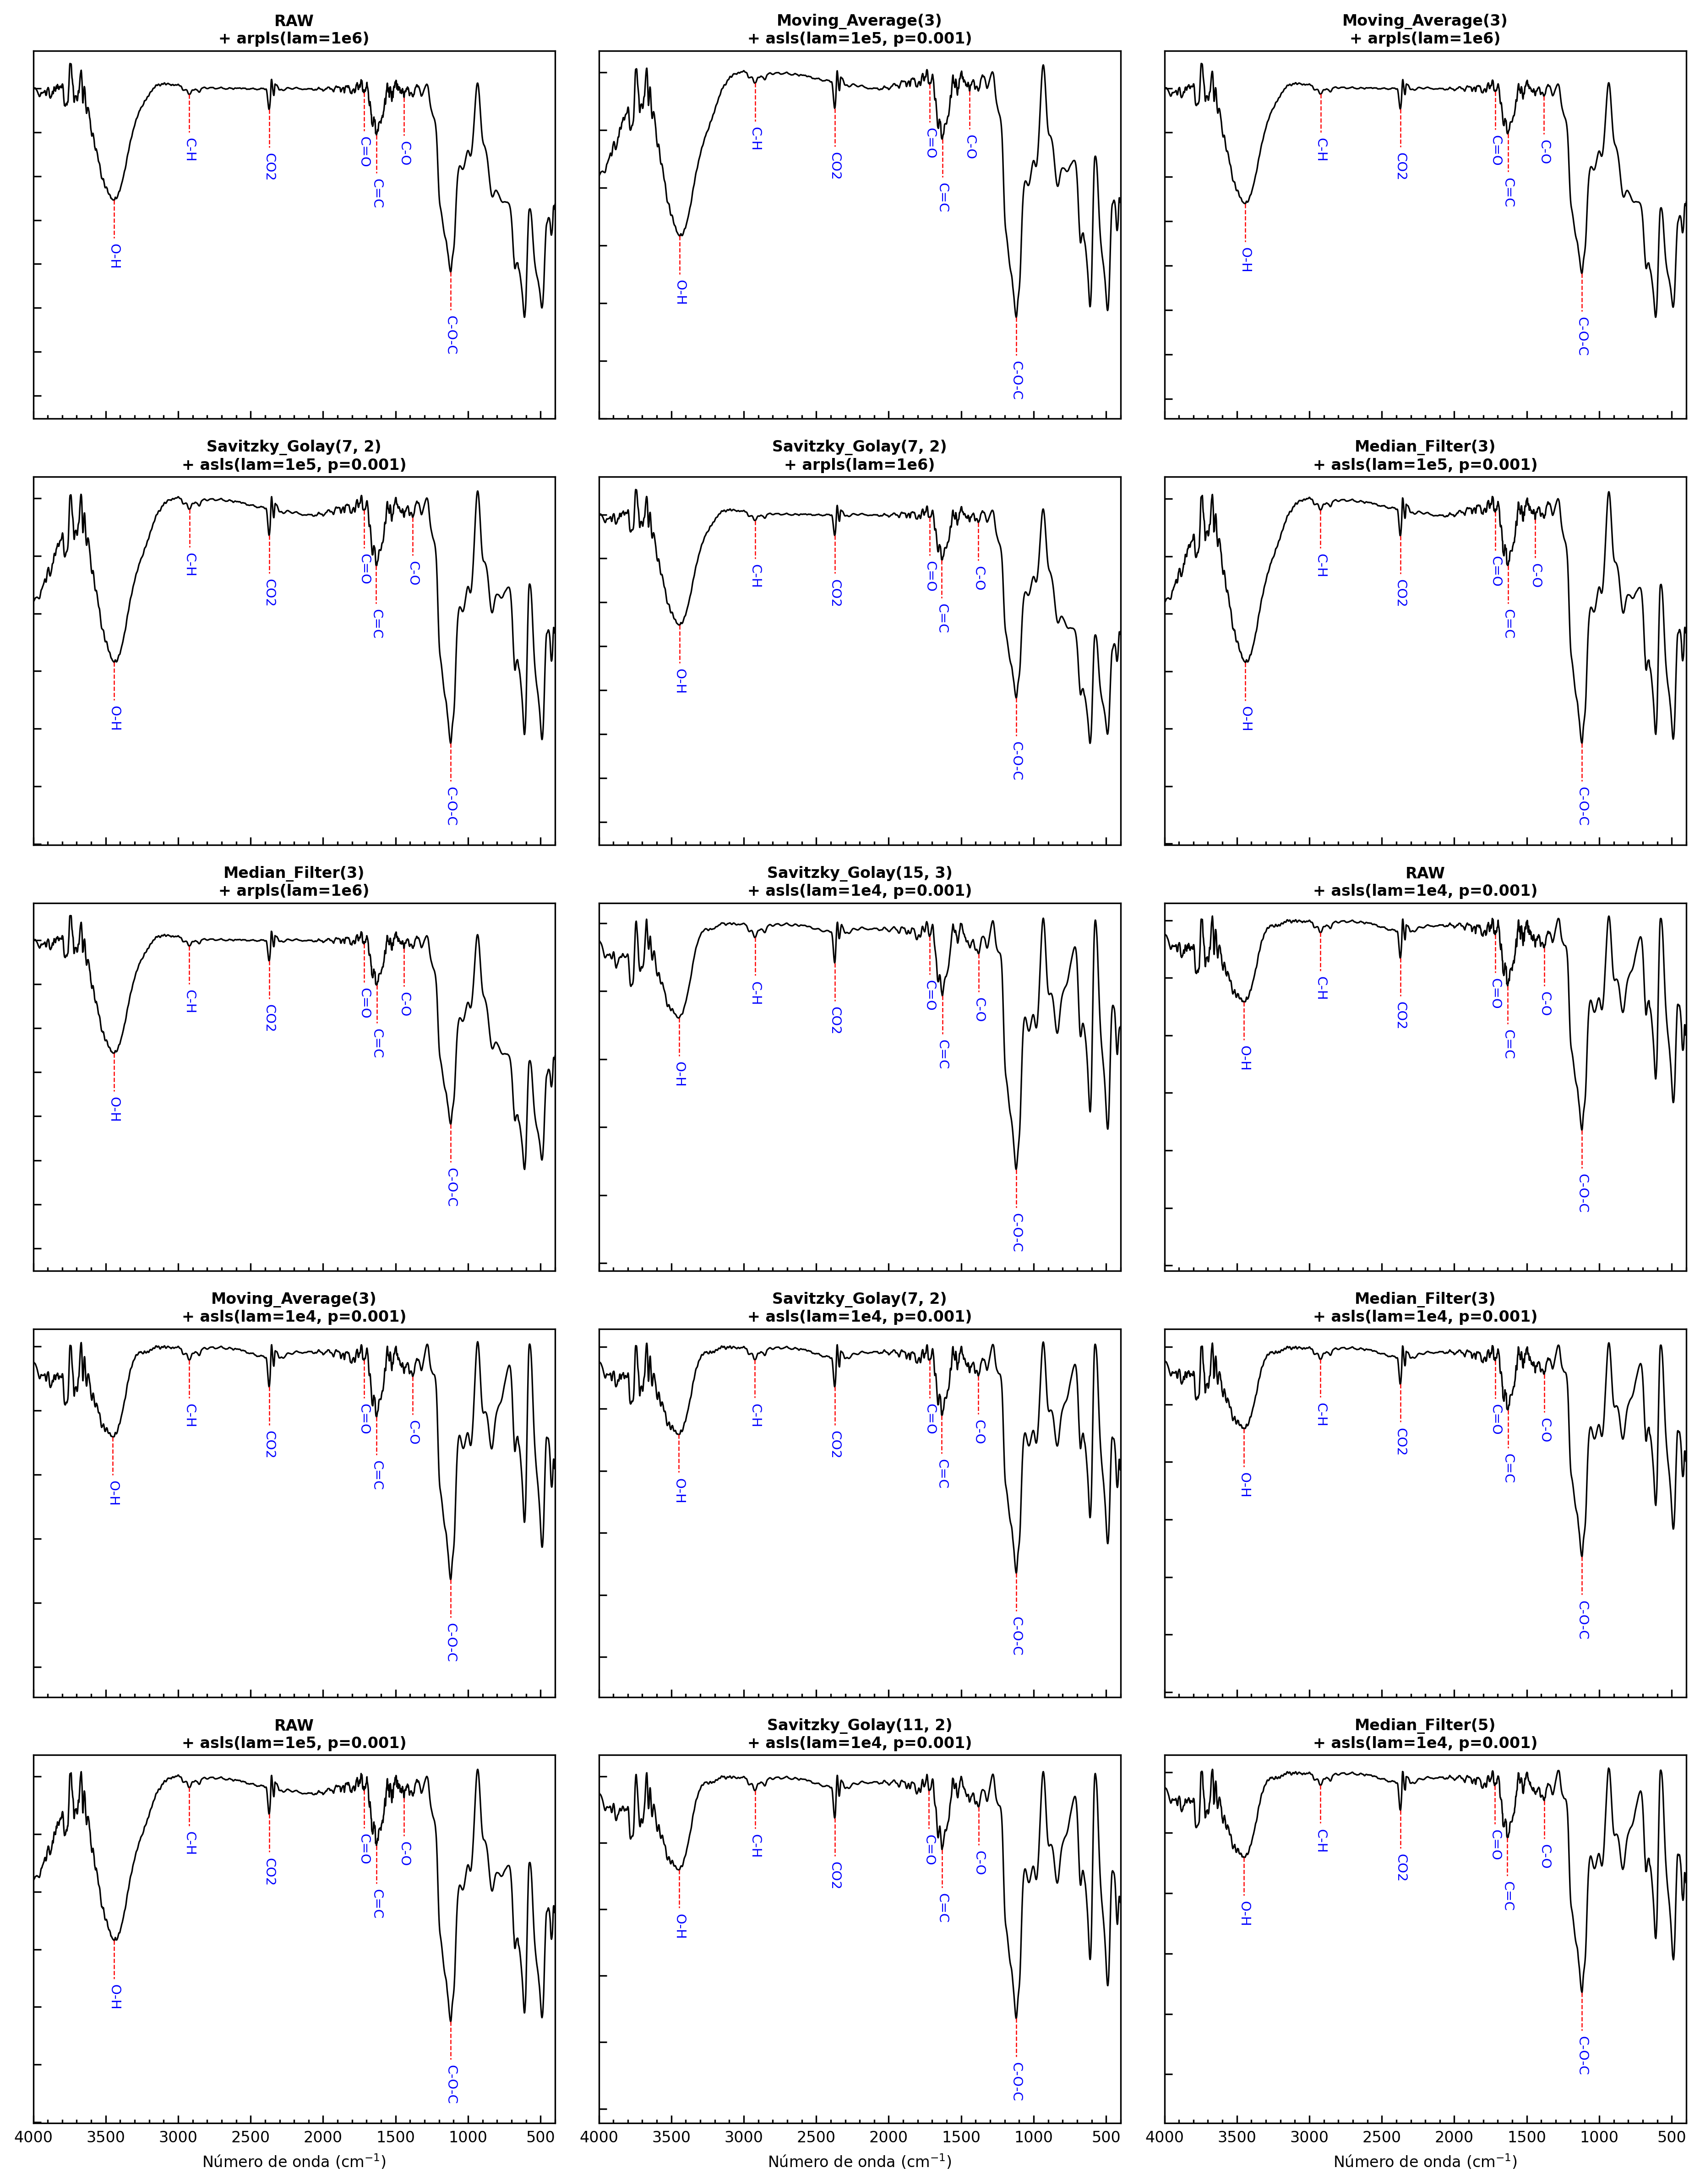
\includegraphics[width=0.85\textwidth]{resultado_galeria_rGO.png}
    \caption{Galería de configuraciones óptimas en Transmitancia para rGO.}
    \label{fig:galeria_trans_rgo}
\end{figure}

\subsubsection{Superposición Comparativa en Transmitancia}
Para evaluar cualitativamente el proceso de reducción mediante transmitancia, se superponen los espectros corregidos óptimos de ambas muestras utilizando el siguiente snippet:

\begin{lstlisting}[language=Python, caption=Superposición de Curvas en Transmitancia]
from ftir_library import plot_superposition

# y_go_corr y y_rgo_corr preprocesados de manera independiente
plot_superposition(
    x_go, y_go_corr, 'Óxido de Grafeno (GO)',
    x_rgo, y_rgo_corr, 'Óxido de Grafeno Reducido (rGO)',
    'images/resultado_superposicion_GO_rGO.png', space='transmittance'
)
\end{lstlisting}

La superposición gráfica resultante se ilustra en la figura \ref{fig:super_trans}, evidenciando la caída drástica en la transmitancia de los picos asociados a los grupos hidroxilo y epóxido tras el tratamiento reductor.

\begin{figure}[h]
    \centering
    
\includegraphics[width=0.7\textwidth]{resultado_superposicion_GO_rGO.png}
    \caption{Superposición de espectros de GO y rGO en Transmitancia.}
    \label{fig:super_trans}
\end{figure}

\newpage

\subsection{Resultados y Gráficos en Espacio de Absorbancia (A)}
El análisis en Absorbancia representa la aproximación físicamente más robusta y simétrica, ya que linealiza la atenuación de la radiación infrarroja y convierte las correcciones de línea base en sustracciones aditivas.

\subsubsection{Preprocesamiento y Búsqueda en Cuadrícula en Absorbancia}
La tubería completa que transforma la transmitancia a absorbancia, corre el grid search de 180 combinaciones y grafica el mejor espectro, se ejecuta mediante el siguiente código:

\begin{lstlisting}[language=Python, caption=Tubería de Preprocesamiento y Graficación Óptima (Absorbancia)]
from ftir_library import (
    load_ftir_data, transmittance_to_absorbance, 
    run_grid_search, plot_best_configuration
)

# Cargar y convertir rGO
x_rgo, y_trans = load_ftir_data("GO coque s lav red.txt")
y_abs = transmittance_to_absorbance(y_trans)

# Búsqueda óptima
best_rgo, results = run_grid_search(x_rgo, y_abs, output_csv="absorbance_pipeline_results_rGO.csv", space="absorbance")

# Graficar óptimo
plot_best_configuration(x_rgo, y_abs, best_rgo, "images/absorbance_result_best_rGO.png", space="absorbance")
\end{lstlisting}

Tras el barrido de 180 configuraciones en Absorbancia, se obtuvieron las siguientes configuraciones de máximo score penalized:
\begin{itemize}
    \item \textbf{Muestra rGO}: \texttt{Percentile\_Filter(5, 75) + airpls(lam=1e4)}, detectando los 7 grupos analíticos y reportando 7 picos válidos (figura \ref{fig:best_abs_rgo}).
    \item \textbf{Muestra GO}: \texttt{Moving\_Average(3) + polynomial\_baseline(deg=4)}, detectando 6 grupos principales (figura \ref{fig:best_abs_go}).
\end{itemize}

\begin{figure}[h]
    \centering
    \begin{minipage}{0.48\textwidth}
        \centering
        \includegraphics[width=\textwidth]{absorbance_result_best_GO.png}
        \caption{Espectro óptimo de GO en Absorbancia.}
        \label{fig:best_abs_go}
    \end{minipage}
    \hfill
    \begin{minipage}{0.48\textwidth}
        \centering
        \includegraphics[width=\textwidth]{absorbance_result_best_rGO.png}
        \caption{Espectro óptimo de rGO en Absorbancia.}
        \label{fig:best_abs_rgo}
    \end{minipage}
\end{figure}

\subsubsection{Galería Modular en Absorbancia (Lotes de 3x1)}
El algoritmo modular implementado genera múltiples imágenes horizontales de 3 columnas para evitar problemas de escala en la impresión:

\begin{lstlisting}[language=Python, caption=Generación de Galerías Modularizadas 3x1]
from ftir_library import plot_gallery_3x1

# Genera lote de imágenes individuales part1.png, part2.png...
plot_gallery_3x1(x_go, y_go_abs, results_go, "images/absorbance_result_gallery_GO", space="absorbance")
\end{lstlisting}

En la figura \ref{fig:galeria_abs_go} se presenta la primera parte de la galería de configuraciones óptimas en Absorbancia para GO, demostrando una excelente legibilidad tipográfica y de ejes en formato A4 horizontal.

\begin{figure}[h]
    \centering
    \includegraphics[width=0.9\textwidth]{absorbance_result_gallery_GO_part1.png}
    \caption{Primera parte ($3 \times 1$) de la galería de configuraciones óptimas en Absorbancia para GO.}
    \label{fig:galeria_abs_go}
\end{figure}

\subsubsection{Superposición Comparativa y Discusión Química en Absorbancia}
La superposición de absorbancias (figura \ref{fig:super_abs}) representa de forma cuantitativa el cambio de absorbancia tras el proceso de reducción química:

\begin{lstlisting}[language=Python, caption=Superposición de Curvas en Absorbancia]
from ftir_library import plot_superposition

plot_superposition(
    x_go, y_go_corr, 'Óxido de Grafeno (GO)',
    x_rgo, y_rgo_corr, 'Óxido de Grafeno Reducido (rGO)',
    'images/absorbance_superposition_GO_rGO.png', space='absorbance'
)
\end{lstlisting}

\begin{figure}[h]
    \centering
    \includegraphics[width=0.7\textwidth]{absorbance_superposition_GO_rGO.png}
    \caption{Superposición comparativa de absorbancia de GO y rGO.}
    \label{fig:super_abs}
\end{figure}

La comparación en el espacio físico de Absorbancia evidencia claramente:
\begin{enumerate}
    \item \textbf{Banda O-H (~3400 cm⁻¹)}: Disminución radical debida a la deshidratación y remoción de los grupos hidroxilo en rGO.
    \item \textbf{Banda C=O (~1720 cm⁻¹)}: Caída notable de los grupos carbonilo presentes en los bordes de la lámina de GO.
    \item \textbf{Banda C=C (~1620 cm⁻¹)}: Estrechamiento e incremento relativo en la absorbancia del enlace aromático en rGO, lo cual evidencia la restauración del plano grafénico $sp^2$.
    \item \textbf{Región Epóxido/Éter C-O-C (~1050 cm⁻¹)}: La remoción casi total del pico epoxi, confirmando la deoxigenación interfacial.
\end{enumerate}

Este comportamiento es consistente con la literatura \cite{silva2021} y valida la exactitud cuantitativa del software desarrollado.


\newpage

% ==========================================
\section{Manual de Usuario: Instalación y Recreación de Pruebas}
% ==========================================
Este manual detalla los pasos requeridos para instalar localmente la biblioteca \texttt{ftir\_library} en Python y recrear de forma automática todas las pruebas, análisis y gráficos presentados en este informe.

\subsection{Instalación de la Biblioteca con Pip}
La biblioteca se distribuye como un paquete comprimido en un archivo ZIP (\texttt{ftirlib.zip}) que contiene todo el código fuente, ejemplos y documentación. El personal del laboratorio puede instalar esta biblioteca directamente desde el archivo ZIP utilizando \texttt{pip} sin necesidad de configurar carpetas de desarrollo.

Para realizar la instalación inicial, abra una terminal o consola de comandos en el directorio donde guardó el archivo \texttt{ftirlib.zip} y ejecute el siguiente comando:

\begin{lstlisting}[language=bash]
# Instalacion inicial desde el archivo ZIP
pip install ftirlib.zip
\end{lstlisting}

Este comando instalará automáticamente la biblioteca y todas sus dependencias necesarias (\texttt{numpy}, \texttt{scipy}, \texttt{matplotlib}) en el sistema.

\subsection{Actualización de la Biblioteca}
En caso de recibir una nueva versión actualizada de la biblioteca por correo electrónico (con el mismo nombre de archivo \texttt{ftirlib.zip}), puede forzar la reinstalación y actualización del paquete ejecutando el comando de reinstalación forzada de \texttt{pip}:

\begin{lstlisting}[language=bash]
# Forzar la reinstalacion y actualizacion de la biblioteca
pip install --force-reinstall ftirlib.zip
\end{lstlisting}

Esto asegura que la biblioteca anterior sea reemplazada completamente por la versión actualizada sin generar conflictos en el sistema.

\subsection{Estructura del Proyecto y Recreación de Pruebas}
Una vez completada la instalación, navegue a la carpeta \texttt{examples/} para ejecutar los scripts de simulación y graficación:

\begin{lstlisting}[language=bash]
# Cambiar al directorio de ejemplos
cd examples
\end{lstlisting}

Los scripts de prueba y sus funciones son los siguientes:

\begin{enumerate}
    \item \textbf{Tubería de Búsqueda y Gráficos Individuales}:
    Ejecute el script que procesa ambas muestras, escribe las tablas de resultados y genera los gráficos óptimos y galerías:
    \begin{lstlisting}[language=bash]
    python run_pipeline_absorbance.py
    \end{lstlisting}
    Este script produce:
    \begin{itemize}
        \item \texttt{absorbance\_pipeline\_results\_rGO.csv} y \texttt{absorbance\_pipeline\_results\_GO.csv}: El historial de las 180 combinaciones por muestra.
        \item \texttt{absorbance\_result\_best\_rGO.png} y \texttt{absorbance\_result\_best\_GO.png}: Gráficos de absorbancia corregida, con líneas punteadas rojas indicadoras y etiquetas azules verticales espaciadas dinámicamente para evitar solapamientos.
        \item \texttt{absorbance\_result\_gallery\_rGO\_partN.png} y \texttt{absorbance\_result\_gallery\_GO\_partN.png}: Grillas horizontales de 3 columnas (en lotes individuales de $3 \times 1$) mostrando las configuraciones que lograron máxima clasificación, optimizadas para impresión en formato A4 sin recortes.
    \end{itemize}

    \item \textbf{Superposición de Curvas Comparativas}:
    Ejecute el script de superposición para generar la gráfica conjunta de comparación:
    \begin{lstlisting}[language=bash]
    python plot_superposition_absorbance.py
    \end{lstlisting}
    Genera el archivo \texttt{absorbance\_superposition\_GO\_rGO.png}.

    \item \textbf{Exportación de Reportes Numéricos Cuantitativos}:
    Genere los reportes CSV que desglosan la posición e intensidad de cada pico y valle de transición analítico:
    \begin{lstlisting}[language=bash]
    python generate_reports.py
    \end{lstlisting}
    Genera los archivos \texttt{report\_peaks\_valleys\_rGO.csv} y \texttt{report\_peaks\_valleys\_GO.csv}, ideales para importar a Excel u otras hojas de cálculo.
\end{enumerate}

% ==========================================
\section{Conclusiones}
% ==========================================
La biblioteca de procesamiento desarrollada en Python y documentada matemáticamente en este reporte demuestra una alta fidelidad para el análisis automático de óxido de grafeno en sus formas oxidada y reducida. La conversión al espacio físico de Absorbancia ha permitido linealizar las correcciones aditivas, mejorando sustancialmente el ajuste de líneas base robustas como AsLS y airPLS.

% ==========================================
\begin{thebibliography}{9}
% ==========================================
\bibitem{savitzky1964}
Savitzky, A., \& Golay, M. J. E. (1964). Smoothing and Differentiation of Data by Simplified Least Squares Procedures. \textit{Analytical Chemistry}, 36(8), 1627-1639.

\bibitem{eilers2003}
Eilers, P. H. C. (2003). A Perfect Smoother. \textit{Analytical Chemistry}, 75(14), 3631-3636.

\bibitem{zhang2010}
Zhang, Z.-M., Chen, S., \& Liang, Y.-Z. (2010). An intelligent background correction method for vibrational spectroscopy. \textit{Analyst}, 135(9), 2338-2346.

\bibitem{baek2015}
Baek, S.-J., Park, A., Shen, Y.-J., \& Lim, J. (2015). A simple and effective baseline correction method for Raman spectra. \textit{Analyst}, 140(1), 250-257.

\bibitem{silva2021}
Silva, M., Rocha Santos Lemos, B., \& Viana, M. (2021). Estudo das propriedades reológicas de nanofluidos à base de etilenoglicol e óxido de grafeno. \textit{Revista de Engenharia e Tecnologia}, 13(2), 1-12.
\end{thebibliography}

\end{document}

